\documentclass{ximera}
\input{../preamble}
\addPrintStyle{..}
\begin{document}
	\author{Zomercursus KU Leuven}
	\xmtitle{Het complexe vlak}{Een meetkundige voorstelling van de complexe getallen}
	\label{xim:cmplx_definitie_complexe_vlak}

Een complex getal $z=a+bi\in \C$ kan worden beschouwd als een punt in het reële  vlak, namelijk als het punt met cartesiaanse coördinaten $(a,b)$, waarbij $a,b$ reële getallen zijn. 
De schrijfwijze $a+bi$ van een complex getal noemt men de \textbf{cartesiaanse vorm}.
We spreken in deze context ook van \textbf{het complexe vlak} of \textbf{het vlak van Gauss}.

\begin{image}[0.3\textwidth]
	\begin{tikzpicture}[scale=3]%,cap=round,transform canvas={scale=0.5}]
	
	\tikzmath{\hoek = 35; \myc = cos(\hoek); \mys = sin(\hoek); 
		\hoekb = 20;}
	
		% Goniometrische cirkel
%	\draw (0,0) circle (1cm);
	\draw[->] (-0.1,0) -- (1.2,0) node[above] {$\Re(z)$};
	\draw[->] (0,-0.1) -- (0,1) node[right] {$\Im(z)$};

	\draw[color=blue,thick] (0:0)  -- (\hoek:1); 
	%
	\draw[color=black] (\hoek:1) node[name=P,circle, fill=black, radius=1pt,scale=0.8] {} node [yshift=2pt,above] {$z=a+bi$} ;  
	%
	\draw[dashed] ({cos(\hoek)},0) node[circle, fill=black, radius=1pt,scale=0.5] {} node[below] {$a$} -- (P);
	\draw[dashed] (0,{sin(\hoek)}) node[circle, fill=black, radius=1pt,scale=0.5] {} node[left] {$b$} -- (P);
	%
	\draw [thick, red,decorate,decoration={brace,amplitude=10pt,mirror},yshift=-5pt](0,0) -- ({cos(\hoek)},0) node[black,midway,yshift=-0.6cm] {\footnotesize $a$};
	%
	\draw [thick, red,decorate,decoration={brace,amplitude=10pt},xshift=-5pt](0,0) -- (0,{sin(\hoek)}) node[black,midway,left,xshift=-8pt] {\footnotesize $b$};
	
	\end{tikzpicture}

\end{image}

De \textbf{zuiver reële} getallen bevinden zich op de (horizontale) $x-$as, die we dan ook de \textbf{reële as} noemen.
\\
De \textbf{zuiver imaginaire} getallen bevinden zich op de (verticale) $y-$as, die we de \textbf{imaginaire as} noemen.

Complexe getallen als punten in het complexe vlak zullen ook een meetkundige interpretatie geven aan de bewerkingen (optellen, vermenigvuldigen, ...) die je met getallen kan uitvoeren. 

% Door deze voorstelling van een complex getal in een vlak kan je ook meetkundig redeneren bij de bewerkingen met complexe getallen. Zo komt de optelling overeen met de optelling van vectoren volgens de regel van het parallellogram. Vermenigvuldigen met $i$ is hetzelfde als een rotatie met $90$ graden. Daaruit volgt dat het kwadraat van $i$ overeenkomt met een rotatie van $180$ graden, en dat is precies hetzelfde als vermenigvuldigen met $-1$. In die zin is $i$ dus wel degelijk een vierkantswortel uit $-1$. Het blijkt dadelijk dat ook $-i$ een vierkantswortel is van $i$.


%nodes goedzetten als compiler terug werkt 

\begin{image}[0.5\textwidth]
	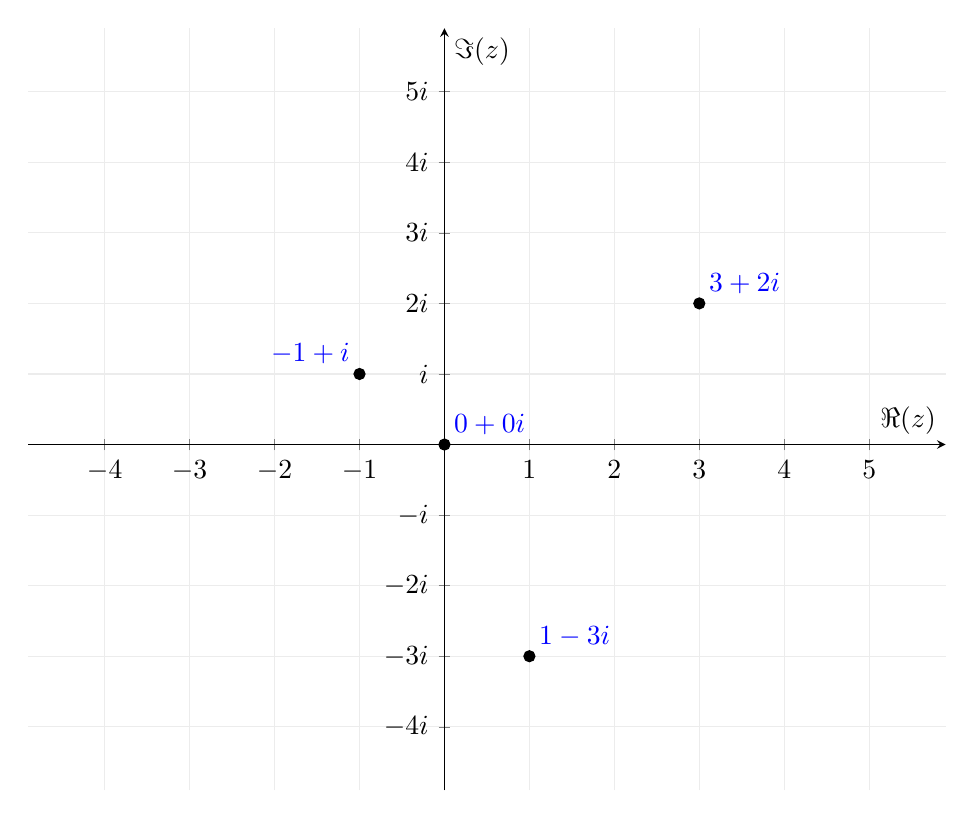
\begin{tikzpicture}
	\begin{axis}
	[
	ytick ={-7,...,8}, yticklabels={$-7i$, $-6i$, $-5i$, $-4i$, $-3i$, $-2i$, $-i$, $0$, $i$, $2i$, $3i$, $4i$, $5i$, $6i$, $7i$, $8i$},
	xtick ={-7,...,8},
	axis lines = center, 
	enlargelimits,
	grid=both,
	grid style={gray!15},
	% minor tick num=1,
	ticks=both,
	xlabel=$\Re(z)$,
	ylabel=$\Im(z)$,
	ymin=-4,
	ymax=+5,
	xmin=-4,
	xmax=+5,
	scale = 1.7,
	]
	
	\addplot [black, mark = *] coordinates {( 0, 0)} {};
	\addplot [black, mark = *] coordinates {( 3, 2)} {};
	\addplot [black, mark = *] coordinates {( -1, 1)} {};
	\addplot [black, mark = *] coordinates {( 1, -3)} {};
	

	\node [above right, blue] at (axis cs:  0, 0) {\(0+0i\)};
	\node [above right, blue] at (axis cs:  3, 2) {$3+2i$};
	\node [above left , blue] at (axis cs: -1, 1) {$-1+i$};
	\node [above right, blue] at (axis cs:  1,-3) {$1-3i$};

	
	\end{axis}
	\end{tikzpicture}
	\qquad



\end{image}


\begin{exercise} Geef devolgende complexe getallen weer als punten in het bovenstaande complexe vlak. 

\begin{xmmulticols}[2]

	\begin{enumerate}
		\item \(3+3i\)
		\item \(-4-4i\)
		\item \(-2i\)
		\item \(4+0i\)
		\item \(-3-4i\)
		\item \(2+5i\)

	\end{enumerate}
	
\end{xmmulticols}

\end{exercise}



\begin{exercise}
    Schets in het complexe vlak de gebieden omschreven door volgende vergelijkingen:
    \begin{question} 
        $\text{Im}(z) \leq 0$
        \begin{oplossing} Als $z=a+bi$, dan betekent Im$(z) \leq 0$ dat $b \leq 0$ en dat geeft het  halfvlak onder de $x$-as:
            \begin{image}[0.2\textwidth]
                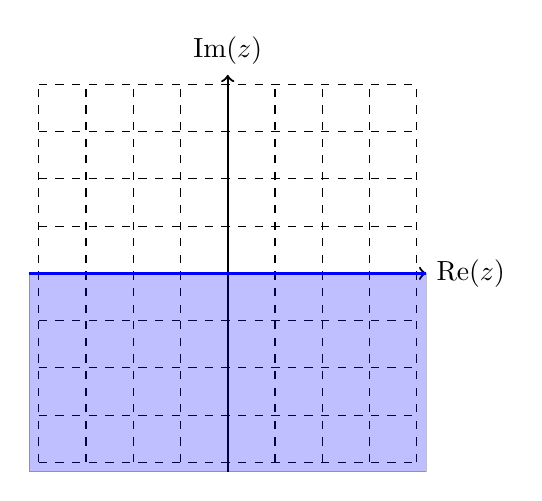
\begin{tikzpicture}[scale=0.6]
                \draw[dashed] (-4, -4) grid (4, 4);
                
                \draw[->, thick] (-4.2, 0) -- (4.2, 0) node[right] {Re$(z)$};
                \draw[->, thick] (0, -4.2) -- (0, 4.2) node[above] {Im$(z)$};
                
                \draw[fill=blue, opacity=0.25] (-4.2,-4.2) rectangle (4.2,0);
                
                % randen toevoegen voor duidelijkheid 
                \draw[blue, very thick] (-4.2,0) -- (4.2,0);
                \end{tikzpicture}
            \end{image}
			
        \end{oplossing}
    \end{question}
    
    \begin{question} 
        $0 \leq \text{Re}(z) \leq 2$
        \begin{oplossing} Deze ongelijkheden bepalen een \textit{verticale} strook, aangezien het reële deel van het complex getal in een interval moet liggen. De randen van de strook behoren tot het geschetste domein.
            
            \begin{image}[0.2\textwidth]
                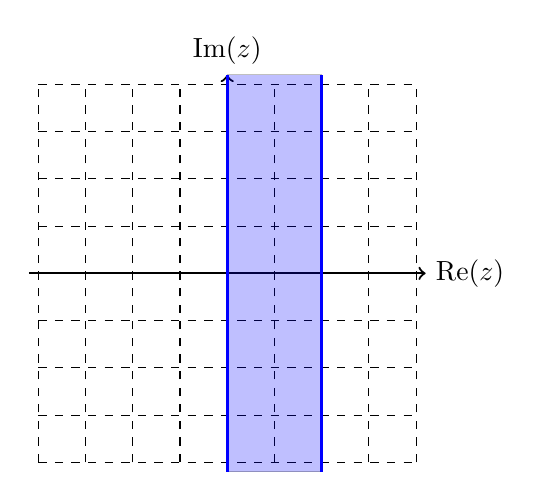
\begin{tikzpicture}[scale=0.6]
                \draw[dashed] (-4, -4) grid (4, 4);
                
                \draw[->, thick] (-4.2, 0) -- (4.2, 0) node[right] {Re$(z)$};
                \draw[->, thick] (0, -4.2) -- (0, 4.2) node[above] {Im$(z)$};
                
                \draw[fill=blue, opacity=0.25] (0,4.2) rectangle (2, -4.2);
                
                % randen toevoegen voor duidelijkheid 
                \draw[blue, very thick] (0, -4.2) -- (0, 4.2);
                \draw[blue, very thick] (2, -4.2) -- (2, 4.2);
                \end{tikzpicture}
            \end{image}
        \end{oplossing}            
    \end{question}        
\end{exercise}




\end{document}
